%% LyX 2.2.3 created this file.  For more info, see http://www.lyx.org/.
%% Do not edit unless you really know what you are doing.
\documentclass[english]{article}
\usepackage[T1]{fontenc}
\usepackage[utf8]{inputenc}
\usepackage{geometry}
\geometry{verbose,rmargin=3cm,bmargin=2cm, footskip=1cm, tmargin=2cm}
\usepackage{float}
\usepackage{textcomp}
\usepackage{graphicx}
\usepackage{verbatim}
\usepackage{amsmath}
\usepackage{hyperref}
\usepackage{datetime}
\usepackage[italian]{babel}
\hypersetup{colorlinks=true}
\usepackage{color}
\definecolor{myred}{rgb}{1,0.98,0.98}
\makeatletter

%%%%%%%%%%%%%%%%%%%%%%%%%%%%%% LyX specific LaTeX commands.
%% Because html converters don't know tabularnewline
\providecommand{\tabularnewline}{\\}

\@ifundefined{date}{}{\date{}}
%%%%%%%%%%%%%%%%%%%%%%%%%%%%%% User specified LaTeX commands.

\usepackage{array}
\usepackage{color}
\usepackage{colortbl}

\makeatother

\usepackage{babel}
\usepackage{listings}
\renewcommand{\lstlistingname}{Listing}

\title{Tutorato Architettura degli Elaboratori Modulo 2 \\ Lezione 2}
\author{Francesco Pelosin}
%\date{4 Aprile 2019}
\date{\today}

\begin{document}
\lstset{frame=single, numbers=left, backgroundcolor=\color{myred}}
\maketitle

\section{Caching}

\begin{figure}[H]
    \centering
   
    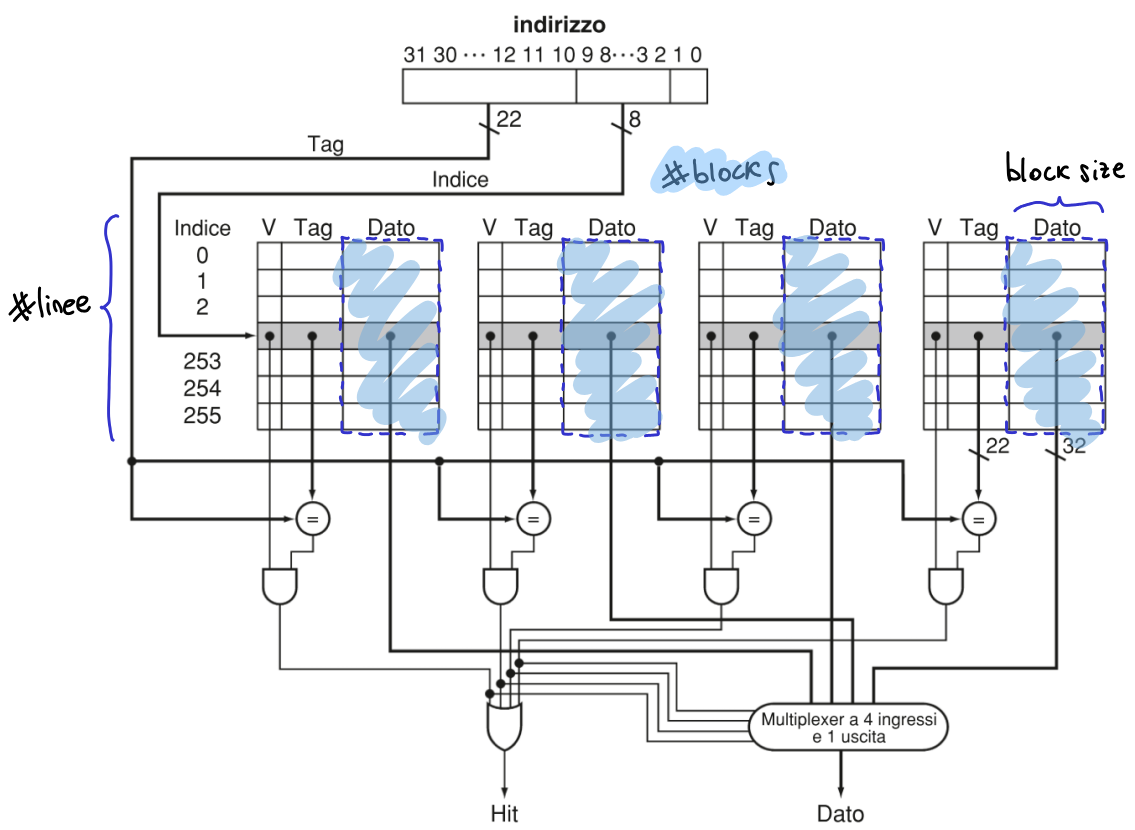
\includegraphics[width=0.95\textwidth]{cache.png}
     
\includegraphics[width=0.5\textwidth]{assoc.png}
    \caption{Esempio 4-way associative cache + reminder associatività}
\end{figure}


\subsection*{Esercizio 1}

I seguenti gruppi di bit degli indirizzi su 32 bit, suddivisi nei diversi campi, vengono utilizzati per l’accesso a una cache a mappatura diretta.

\begin{table}[H]
\centering
\begin{tabular}{|c|c|c|}
\hline
\textbf{Tag} & \textbf{Index} & \textbf{Offset} \\ \hline
31-10        & 9-5            & 4-0             \\ \hline
\end{tabular}
\end{table}

\begin{enumerate}
    \item Quanti blocchi contiene la cache?
    \item Qual è la dimensione di un blocco della cache (in numero di words)?
    \item Qual è il rapporto tra il numero totale di bit contenuti in questa cache e il numero di bit utilizzati per memorizzare i dati?

%   \item A partire dall’accensione del calcolatore, si verifca una sequenza di accessi alla cache con i seguenti indirizzi, riferiti al byte:
%
%\begin{table}[H]
%\centering
%\begin{tabular}{|c|c|l|l|l|l|l|l|l|l|l|l|}
%\hline
%\multicolumn{12}{|c|}{\textbf{Indirizzo}}                          \\ \hline
%0 & 4 & 16 & 132 & 232 & 160 & 1024 & 30 & 140 & 3100 & 180 & 2180 \\ \hline
%\end{tabular}
%\end{table}
%
%    \begin{enumerate}
%        \item Quanti blocchi vengono sostituiti?
%        \item Qual è la frequenza di hit?
%        \item Riportare lo stato fnale della cache, indicando (per ogni blocco che contiene un dato valido) indice, \texttt{Ta e dato contenuto.
%    \end{enumerate}

\end{enumerate}

\subsubsection*{Soluzione}

\begin{enumerate}
    \item La composizione degli indirizzi è la seguente:
    \begin{itemize}
        \item \texttt{OFFSET}: 5 bit
        \item \texttt{INDEX}: 5 bit
        \item \texttt{TAG}: 22 bit
    \end{itemize}
    Essendo la cache ad accesso diretto, abbiamo che il numero di blocchi della cache corrisponde al numero delle entrate (linee). Quindi $2^{5}=32$ blocchi della cache.
    
    \item Siccome abbiamo 5 bit di \texttt{OFFSET} ogni blocco contiene $2^{5} = 32$ Byte (ricordiamo che l'indirizzamento nel MIPS avviene al Byte). Abbiamo quindi $2^{5} \cdot 2^{3} = 2^{8}$ bit totali per ogni blocco della cache. Ossia, passando da bit a words, abbiamo $2^{8}/32 = 8$ words per blocco.
    \item I dati contenuti nella cache sono: $2^{5} \cdot 2^{5}$ Byte ossia $2^{5} \cdot 2^{5} \cdot 2^{3} = 2^{13}$ bit che corrispondono a 8 kB. Per ricavare la quantità di dati necessari per la memorizzazione, dobbiamo moltiplicare i bit di \texttt{TAG} e di Validità per il numero di blocchi della cache. Ossia $2^{5} \cdot (22 + 1) = 736$ bit. Abbiamo quindi che la dimensione totale è $(2^{13} + 736) / 2^{13} = 1.0898$ volte la dimensione dei soli dati.
\end{enumerate}


\subsection*{Esercizio 2}
Considerare due cache la cui parte dati è di dimensione 128 kB, con blocchi di 64 bit. Dato un indirizzo fisico di 32 bit, determinare le organizzazioni (suddivisione dei bit dell'indirizzo e livello di associatività) delle cache per dimensioni della \texttt{TAG} di 16 bit e di 18 bit.

\subsubsection*{Soluzione}

\paragraph{Tag 16 bit}

Abbiamo che ogni blocco contiene 64 bit ($2^{6}$ bit) ossia 8 Byte ($2^{3} \cdot 2^{3}$ bit). Ricordando che l'indirizzamento nel blocco nel MIPS si effettua al Byte, avremo che il campo \texttt{OFFSET} dell'indirizzo sarà composto da 3 bit. Il campo \texttt{INDEX} sarà dunque $32-3-16=13$ bit. Significa che vi saranno presenti $2^{13}$ linee della cache.

Per quanto riguarda il livello di associatività, dobbiamo prima ricavare il numero di blocchi della cache. Ricaviamo il numero totale di blocchi dividendo il totale dei dati (128 kB) per la dimensione di un blocco (64 bit). Trasformiamo la scala dei dati da kB a bit nel seguente modo: 128 kB $= (128 \cdot 1024 \cdot 8)$ bit. Ora possiamo calcolare il numero di blocchi: 

$$\#blocchi = \frac{128 \cdot 1024 \cdot 8}{64} = \frac{2^{7} \cdot 2^{10} \cdot 2^{3}}{2^{6}} = 2^{14}$$

Il livello di associatività sarà dato da $2^{14}/2^{13} = 2$. La cache quindi è una 2-way associative cache.

\paragraph{Tag 18 bit}
Il campo \texttt{OFFSET} non cambia e richiede sempre 3 bit. Cambia invece il campo \texttt{INDEX} che sarà formato da $32-3-18=11$ bit. Significa che in questo caso $\#linee = 2^{11}$. 

Il livello di associatività sarà $2^{14} / 2^{11} = 2^{3} = 8$. La cache, dunque, è una 8-way associative cache.

\subsection*{Esercizio 3}

Si supponga di avere una cache con una parte dati di 64 kB, avente blocchi da 16 Byte. L'organizzazione della cache può essere diretta (a) o 2-way associative (b).
\begin{enumerate}
    \item  Calcolare la dimensione dell'\texttt{INDEX}, \texttt{TAG} e \texttt{OFFSET} per il caso (a) e (b).

    \item Rispetto alla cache diretta, si supponga che questa sia all'inizio vuota. Si supponga che un programma faccia riferimento alla memoria con un puntatore $p$, inizialmente $p=\mathrm{0x17100004}$ (indirizzo fisico di 32 bit espresso in esadecimale), via via $p$ viene incrementato del valore $\mathrm{0x00000080}$ (ossia 128 in decimale).  Valutare per quale valore dell'indirizzo (e per quale corrispondente valore di \texttt{INDEX}) si verifica il primo conflitto.

\end{enumerate}

\subsubsection*{Soluzione}

\begin{enumerate}
    \item 
    \begin{enumerate}
   
        \item \textbf{Cache diretta.} Ricaviamo la dimensione della parte dati in bit: 64 kB $= 2^{6} \cdot 2^{10} \cdot 2^{8} = 2^{19}$. Ricaviamo la dimensione del blocco in bit: 16 Byte $= 2^{4} \cdot 2^{3} = 2^{7}$. 
        
        Ora possiamo ricavare il numero di blocchi di cui è composta la cache, nello specifico sarà: $\#blocks = 2^ {19} / 2^{7} = 2^{12} = 4096$ blocchi. Considerando che la cache è diretta abbiamo un blocco per linea quindi la dimensione dell'\texttt{INDEX} sarà di 4096 entrate ossia $2^{12}$ che corrispondono a 12 bit nell'indirizzo. Sappiamo inoltre che la dimensione del singolo blocco è di 16 Byte, sono necessari, dunque, 4 bit di \texttt{OFFSET} per indirizzare il byte corretto nel blocco. Possiamo ora ricavare la dimensione dei bit di \texttt{TAG}, che sarà $32-12-4=16$.

        \item \textbf{2-way associative cache.} In questo caso abbiamo che per ogni linea della cache abbiamo due blocchi, ossia: $2^{7} \cdot 2^{1} = 2^{8}$. Possiamo dunque ricavare il numero delle linee della cache come segue $\#linee = 2^{19} / 2^{8} = 2^{11}$. Per indirizzare $2^{11}$ entries abbiamo bisogno di 11 bit per l'\texttt{INDEX}. La dimensione dei bit dell'\texttt{OFFSET} non cambia mentre la dimensione del \texttt{TAG} diventa 17 bit.
    \end{enumerate}
    
    \item Considerando la cache ad accesso diretto abbiamo che ogni indirizzo è suddiviso nel seguente modo:

    $$\mathrm{0x} \; \underset{_{TAG}}{\underbrace{1710}} \;  \overset{^{INDEX}}{\overbrace{000}} \underset{_{OFFSET}}{\underbrace{4}}$$
    
    Sappiamo che ci sarà un conflitto nella cache quando due blocchi, indicizzati sullo stesso \texttt{INDEX}, vengono acceduti. Il programma accede alla cache con la seguente sequenza di indirizzi fisici:
    
\begin{lstlisting}[numbers=none]
0x 1710 000 4  //INDEX= 0
0x 1710 008 4  //INDEX= 8
0x 1710 010 4  //INDEX=16
0x 1710 018 4  //INDEX=24
0x 1710 020 4  //INDEX=32
0x 1710 028 4  //INDEX=40
0x 1710 030 4  //INDEX=48
0x 1710 038 4  //INDEX=56
0x 1710 040 4  //INDEX=64
...
0x ???? ??? ?  //INDEX= 0  Conflitto! 
\end{lstlisting}
    
    Tenendo conto che l'incremento di 0x80 corrisponde ad un crimento di 8 dell'\texttt{INDEX}, e sapendo che la dimensione della cache è $4096 = 2^{12}$ linee, significa che il numero di accessi prima che si verifichi un conflitto\footnote{Nell'esercizio consideriamo il numero di accessi necessari prima del primo conflitto, più in generale i conflitti sono dati dagli $n$ che soddisfano l'equazione} sarà $n \cdot 2^3 = 2^{12}$ ossia $n=2^{9}=\mathrm{0x200}$.
    
    Tradotto in esadecimale l'indirizzo del primo conflitto sarà:
    
    $$\mathrm{0x17100004} + \mathrm{0x200} \cdot \mathrm{0x80} = \mathrm{0x17100004} + \mathrm{0x10000} = \mathrm{0x17110004}$$

    
\end{enumerate}



\section{Prestazioni Caching}

\begin{figure}[H]
    \centering
    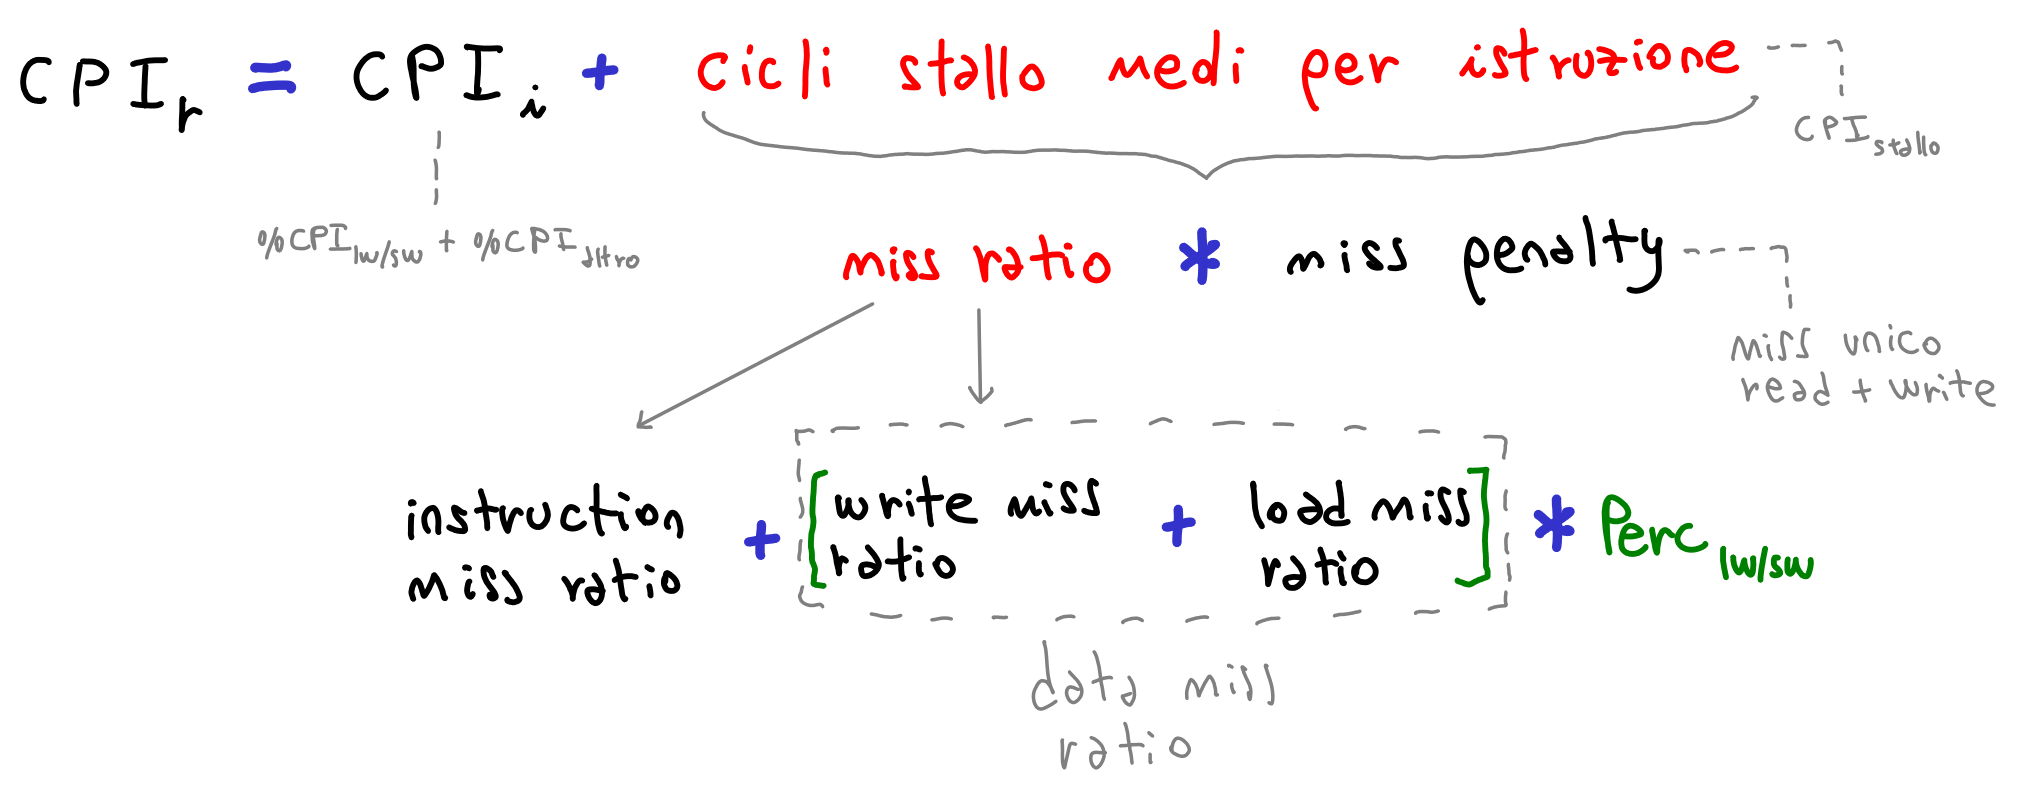
\includegraphics[width=1\textwidth]{cpi.png}
    \caption{Reminder relazione fondamentale.}
\end{figure}



\subsection*{Esercizio 4}
Considerare l’esecuzione di un programma $P$ su di una data CPU. Calcolare il CPI ideale ($CPI_i$), considerando che, senza gli effetti della cache, il CPI medio delle load/store sarebbe 4.5, il CPI medio delle altre istruzioni sarebbe 2, mentre la percentuale di load/store è del 40\%. Considerando i miss della cache si ottiene un CPI reale ($CPI_r$) pari a 3.6. Sapendo che $InstructionMissRate = 4\%$, $DataMissRate = 2.5\%$, determinare il $MissPenalty$ (in cicli).
Calcolare i tempi, reali e ideali, per eseguire $P$, considerando che $IC = 200$ Milioni, mentre la frequenza della CPU è di 500 MHz.


\subsubsection*{Soluzione}

Iniziamo ricavando il $CPI_{i}$ considerando le istruzioni di load/store e le restanti istruzioni.
\begin{equation*}
\begin{aligned}
    CPI_i =& 0.4 \cdot CPI_{lw,sw} + 0.6 \cdot CPI_{altro} \\
          =& (0.4 \cdot 4.5) + (0.6 \cdot 2) = 3
\end{aligned}
\end{equation*}
Per alleggerire la notazione sia $x = MissPenalty$. Abbiamo che:
\begin{equation*}
\begin{aligned}
    CPI_r =& CPI_{i} + 0.04 \cdot x + 0.4 \cdot 0.025 \cdot x \\
      3.6 =& 3 + 0.04 \cdot x + 0.4 \cdot 0.025 \cdot x \\
        x =& \frac{0.6}{0.04 + 0.4 \cdot 0.025} = 12 \text{ cicli}
\end{aligned}
\end{equation*}
Sapendo che la CPU è a 500 MHz, allora:

$$T = \frac{1}{500 \cdot 10^{6}}$$
Il tempo di esecuzione ideale è quindi:

\begin{equation*}
\begin{aligned}
T_{exe_i} =& CPI_{i} \cdot IC \cdot T \\
        =& 3 \cdot 200 \cdot 10^{6} \cdot \frac{1}{500 \cdot 10^{6}} \\
        =& \frac{600}{500} = 1.2 sec.
\end{aligned}
\end{equation*}
Mentre il tempo di esecuzione reale è:
\begin{equation*}
\begin{aligned}
T_{exe} =& CPI_{r} \cdot IC \cdot T \\
        =& 3.6 \cdot 200 \cdot 10^{6} \cdot \frac{1}{500 \cdot 10^{6}} \\
        =& \frac{720}{500} = 1.44 sec.
\end{aligned}
\end{equation*}


\subsection*{Esercizio 5}
Abbiamo le seguenti misure relative all’esecuzione di un certo programma su un processore a 2 GHz:
\begin{itemize}
    \item $CPI_{i} = 2$
    \item $Perc_{lw,sw} = 20\%$
    \item $DataMissRate = 30\%$
    \item $InstructionMissRate = 5\%$
    \item $IC=10$ Milioni
    \item $T_{exe} = 65 ms$
\end{itemize}

\begin{enumerate}
    \item Si richiede di calcolare il $MissPenalty$ espresso in ns.
    \item Modificando la cache, e mantenendo inalterato il resto del sottosistema di memoria, si osserva un miglioramento del $DataMissRate$. Se otteniamo un tempo di esecuzione $T_{exe} = 40ms$, quanto vale il nuovo $DataMissRate$?
\end{enumerate}




\subsubsection*{Soluzione}

\begin{enumerate}
    \item Per alleggerire la notazione poniamo $x = MissPenalty$. 
    
Sappiamo che:

\begin{equation*}
\begin{aligned}
CPI_{stallo} =& (InstructionMissRate + DataMissRate \cdot Perc_{lw,sw}) \cdot x \\
           =& (0.05 + 0.06) x = 0.11 x 
\end{aligned}
\end{equation*}

Possiamo ora ricavare il $CPI_{r}$: 

$$CPI_r = CPI_i + CPI_{stallo} = 2 + 0.11 x$$ 

A questo punto sembrerebbe impossibile ricavare $x$ in quanto non sappiamo quanto è $CPI_{r}$. Guardando bene i dati del problema possiamo sfruttare $T_{exe}$ per proseguire.

Ricordiamo che $T_{exe} = CPI_{r} \cdot  IC \cdot T$ di conseguenza abbiamo:

$$T_{exe}= CPI_{r} \cdot IC \cdot T = (2 + 0.11 x) \cdot 10^{7} \cdot T$$

Ricaviamo $T$ dalla frequenza del processore (2GHz), nel seguente modo:

$$T = \frac{1}{2 \cdot 10^{9}} = 0.5 ns$$

Ora possiamo ricavare $x$ dall'equazione, visto che $T_{exe} = 65ms$. Infatti:

\begin{equation*}
\begin{aligned}
T_{exe} =& CPI_{r} \cdot IC \cdot T \\
65 \cdot 10^{-3} =& (2 + 0.11x) \cdot 10^{7} \cdot 0.5 \cdot 10^{-9} \\
65 =& (2 + 0.11x) \cdot 5 \\
65 =& 10 + 0.55x \\
 x =& \frac{65 - 10}{0.55} = 100 \text{ cicli}
\end{aligned}
\end{equation*}

Per esprimere il miss penalty in $ns$, basta moltiplicare per $T$:

$$MissPenalty \cdot T = 100 \cdot 0.5 ns = 50 ns$$



\item Sia $x$ il nuovo valore del $DataMissRate$:

$$CPI_{stallo} = (InstructionMissRate + x \cdot Perc_{lw,sw}) \cdot MissPenalty = (0.05 + 0.2 x) 100 = 5 + 20x$$

$$CPI_{r} = CPI_{i} + CPI_{stallo} = 2 + (5 + 20 x) = 7 + 20 x$$

Sfruttiamo ancora la definizione di $T_{exe}$.

\begin{equation*}
\begin{aligned}
T^{'}_{exe} =& CPI_{r} \cdot IC \cdot T \\
            =& (7 + 20x) \cdot 10^{7} \cdot 0.5 \cdot 10^{-9} \\
            =& (7 + 20x) \cdot 5 \cdot 10^{6} \cdot 10^{-9} \\
            =& (7 + 20x) \cdot 5 \cdot 10^{-3}
\end{aligned}
\end{equation*}

Metto nell'equazione il tempo di esecuzione dato dalla consegna e calcolo il nuovo $DataMissRate$ risolvendo l’equazione per $x$.

\begin{equation*}
\begin{aligned}
T^{'}_{exe} =& (7 + 20x) \cdot 5 \cdot 10^{-3} \\
40 \cdot 10^{-3} =& 35 \cdot 10^{-3} + 10^{-1} x \\
10^{-1} x =& 5 \cdot 10^{-3} \\
x =& 5 \cdot 10^{-2} = 0.05 = 5\%
\end{aligned}
\end{equation*}
Il nuovo $DataMissRate$ è del 5\%.


\end{enumerate}


\subsection*{Esercizio 6}
Un computer a 1 GHz, nell’eseguire un certo programma, ha una prestazione ideale di 500 MIPS (senza considerare la cache e i miss relativi). 
Considerando la cache, il $CPI_{r}$ misurato diventa uguale a 2.48. Conoscendo che il data e l’instruction miss rate sono entrambi uguali al 2\% e che la percentuale di load/store è del 20\%, si chiede di:

\begin{enumerate}
    \item Calcolare il $CPI_{i}$
    \item Calcolare il $MissPenalty$
\end{enumerate}

\subsubsection*{Soluzione}

\begin{enumerate}
    \item Poiché la prestazione ideale è di 500 MIPS ed il processore è a 1GHz significa che, in media, ci impiegheremmo 2 cicli a completare una istruzione\footnote{La capacità di esecuzione è di 1 miliardo di istruzioni al secondo, se la prestazione ideale prevede 500 milioni di istruzioni al secondo, significa che ogni due cicli finiamo un'instruzione.}.
    
    Possiamo riformulare più formalmente la soluzione, in particolare ricordandoci che :
    
    $$MIPS = \frac{IC}{T_{exe_i} \cdot 10^{6} }$$
    e che: 
    $$T = \frac{1}{F}$$
    abbiamo:
    \begin{equation*}
    \begin{aligned}
    MIPS =& \frac{IC \cdot F}{IC \cdot CPI_{i} \cdot 10^{6}} = \frac{F}{CPI_{i} \cdot 10^{6}} \\
    500 =& \frac{10^{9}}{CPI_{i} \cdot 10^{6}} \\
    500 =& \frac{10^{3}}{CPI_{i}} \\
    CPI_{i} =& \frac{10^{3}}{500} = 2
    \end{aligned}
    \end{equation*}    
    
    \item Quello appena calcolato è il $CPI_{i}$, possiamo dunque ricavare $MissPenalty$ nel seguente modo:
    \begin{equation*}
    \begin{aligned}
    CPI_{stallo} =& CPI_{r} - CPI_{i} \\
                 =& 2.48 - 2 \\
                 =& 0.48
        \end{aligned}
    \end{equation*} 
    Da quì possiamo sfruttare il fatto che $CPI_{stallo} = MissRatio \cdot MissPenalty$ e ricavare $MissPenalty$ attraverso la composizione di $MissRatio$, in particolare:
    \begin{equation*}
    \begin{aligned}
    0.48 =& (2\% + 2\% \cdot 20\%) \cdot MissPenalty \\
    0.48 =& (0.02 + 0.02 \cdot 0.2) \cdot MissPenalty \\
    MissPenalty =& 20
    \end{aligned}
    \end{equation*}  
\end{enumerate}


\section*{Nota Bene: differenze tra kB e KiB}
In questa lezione abbiamo considerato 1 kB $= 2^{10}$ Byte. Qesta NON sarebbe la definizione standard. Si tratta di una convenzione che viene usata comunemente dagli informatici per facilitare i conti. Infatti:

\begin{itemize}
\item Definizione standard: 1 kB $= 1000$ Byte.
\item Definizione NON standard: 1 kB $= 1024$ Byte.

\end{itemize}
Il nome corretto per la definizione non standard sarebbe il kibibyte (KiB). Di fatto, nell'ambito dell'informatica, si scrive impropriamente kB per intendere KiB. Da poco il termine kibibyte sta iniziando ad essere sempre più comune, questo è importante in quanto la differenza tra 1 kB e 1 KiB non è trascurabile (sono 192 bit persi per sempre!). Lo stesso discorso si estende ai MB ed ai MiB e via dicendo.

\section*{Risorse}
\begin{itemize}
    \item Wikipedia: \href{https://it.wikipedia.org/wiki/Chilobyte#Quanto_vale_un_chilobyte?}{kB vs. KiB}, \href{https://it.wikipedia.org/wiki/Prefissi_per_multipli_binari}{prefissi binari vs decimali} 
    \item Struttura e progetto dei calcolatori - David A. Paterson, John L. Hennessy, Capitolo 5. 
\end{itemize}





%\subsection*{Esercizio 1}
%Dati una cache con 4096 blocchi, e con dimensione dell’\texttt{INDEX} di 10 b, determinare il grado di associatività della cache stessa.
%Determinare la dimensione dell’indirizzo fisico, considerando che la \texttt{TAG} è 18 b, mentre la dimensione della parte dati della cache è 64 kB.
%Considerare infine la seguente sequenza di accessi alla memoria (sequenza di %\texttt{lw}):
%
%\begin{lstlisting}
%0x000000a4
%0x000000ac
%0x100000a4
%0x100000ac
%0x200000a4
%0x200000ac
%0x300000a4
%0x300000ac
%0x400000a4
%\end{lstlisting}
%
%Supporre che tutti blocchi della cache siano non validi. Quali accessi provocano hit, miss, oppure miss con conflitto?

%\subsubsection*{Soluzione}
%
%\begin{itemize}
%\item No. di vie = num. blocchi / 2INDEX = 4096 / 1024 = 4.
%\item Dimensione blocco $= \frac{64 kB}{4096} = \frac{2^{16}}{2^{12}} = 2^{4}$
%\item Ind. Fisico = INDEX + \texttt{TAG} + OFFSET $= 10 + 18 + log_2 (Dim\_blocco) = 28 + 4 = 32 b$.
%
%\end{itemize}
%
%
%Per quanto riguarda i nove accessi, i 4 b dell’\texttt{OFFSET} corrispondono alla cifra esadecimale meno significativa dell’indirizzo fisico. Inoltre, bisogna considerare che INDEX, ovvero la parte bassa del block address, ovvero la parte bassa dell’indirizzo fisico una volta eliminato \texttt{OFFSET}, è grande 10 b. Quindi, in tutti e nove i casi INDEX rimane costante. Quindi, tutti e nove gli accessi fanno riferimento al solito INDEX, ovvero allo stesso set a 4 vie. Inoltre le coppie di accessi (1,2), (3,4), (5,6), (7,8) fanno riferimento allo stesso blocco. Infatti, se si considerano gli indirizzi presenti in ogni coppia, si può osservare che cambiano solo i 4 bit meno significativi (l’ultima cifra esadecimale), ovvero l’\texttt{OFFSET}. Gli accessi 1, 3, 5 e 7 sono sicuramente miss, poiché ogni volta cambia il \texttt{TAG} (la parte alta dell’indirizzo). I rispettivi blocchi verranno ospitati in blocchi diversi del set a 4 vie individuato dall’INDEX. Gli accessi 2, 4, 6 e 8 sono invece hit.
%Infine, l’ultimo accesso (il 9) è anch’esso un miss a causa del \texttt{TAG} ancora diverso. Quest’ultimo provoca però un conflitto, poiché tutti e 4 i blocchi del set sono a questo punto occupati.

\end{document}